\chapter{INTRODUCTION}
\label{chap:intro}

The installed capacity of solar power in the US continues to grow as a
result of aging coal and natural gas power plants, lower costs,
state renewable portfolio standards, and efforts to decarbonize the
electrical grid.
As shown in \Cref{fig:solarinstall}, this growth has been steady since
2010 and shows no signs of abating.

\begin{figure}[htb]
  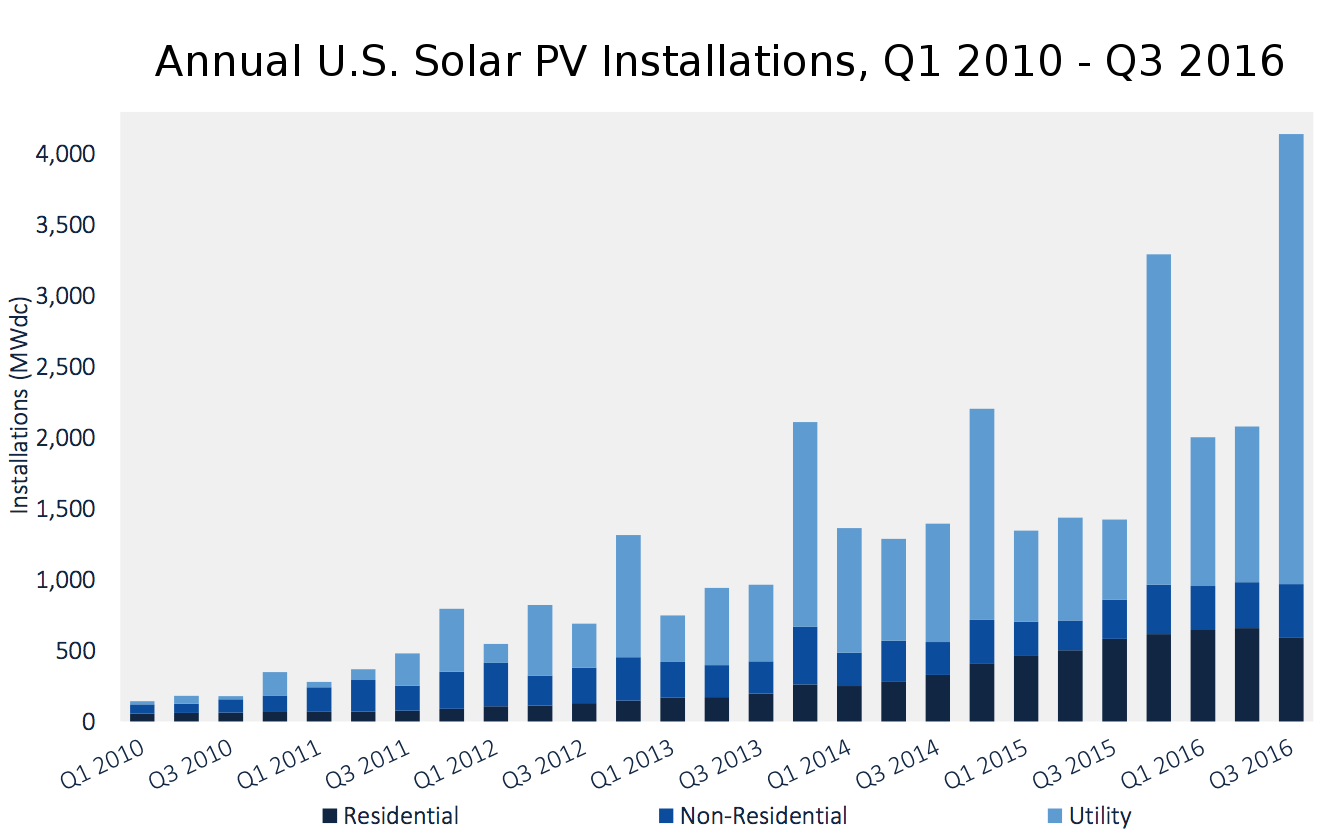
\includegraphics[width=\textwidth]{figs/solar_installations.png}
  \caption[Annual installations of solar PV in the US]{Annual
    installations of solar photovoltaic (PV) systems in the
    US. [Source:~\cite{GTM/SEIA2016}]}
\label{fig:solarinstall}
\end{figure}

Solar irradiance is the fuel that drives all solar power plants.
Unlike sources of fuel for conventional power generators like coal or
natural gas, the solar resource is highly variable due to chaotic
nature fo the weather.
This variability of the solar resource leads to uncertainty at the
electric utility and increases management costs \citep{Joskow2011}.
Forecasts help utilities manage the variability in a number of ways
\citep{Kleissl2013,Inman2013}, including the optimal dispatch of
battery storage \citep{Cormode2015}.
Ultimately, better forecasts increase the amount of solar power that
utilties add to the grid.

This dissertation will explore solar irradiance forecasting techniques
that incorporate data from a ground sensor network.
First, the current state of solar power in the Southwest US and a
brief overview of general irradiance forecasting methods will be
discussed. Then, a brief overview of solar irradiance forecasting
methods will be presented. Finally, a summary of the work in this
dissertation will be proivded.

\section{State of Solar Power in the Southwest and Future Challenges}

As of early 2017, members of the Southwest Variable Energy Resource
Initiative (SVERI) have a total of 1100 MW of installed solar capacity,
800 MW of installed wind capacity, and a peak load of 23 GW
\citep{sveri_website}.
Another roughly 1 GW of generation comes from distributed generation
(DG) solar systems that are installed on residential or commercial
rooftops.
Heatmaps showing the time of day load, wind and solar generation, and
wind and solar fraction of load for two years are shown in
\cref{fig:sveri_heatmap}.
Heatmaps for weather variables at the University of Arizona are shown
in \cref{fig:ua_heatmap} to correlate weather to, for example, the
abrupt decrease in load around 10/14 corresponding to the end of monsoon season.

\begin{figure}[p]
\centering
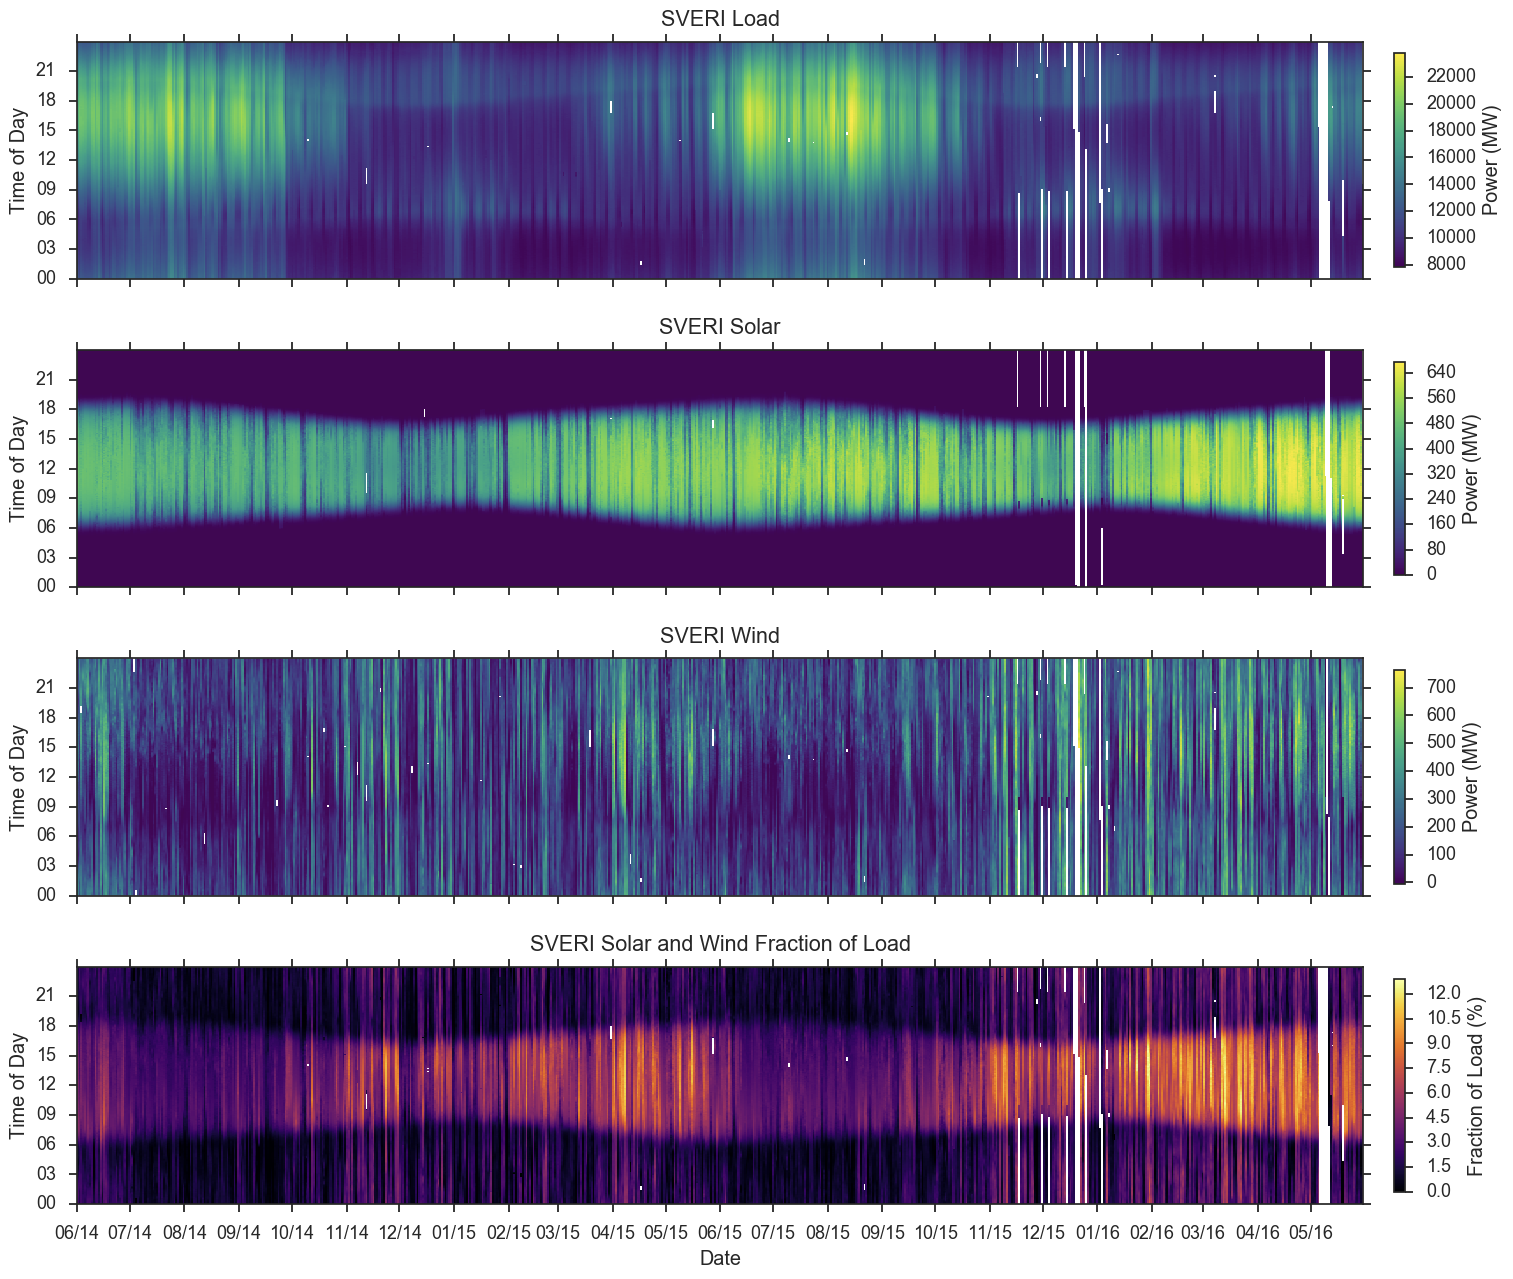
\includegraphics[width=\textwidth]{figs/sveri_heat.png}
\caption[Heatmaps of SVERI load, solar power, wind power, and
renewable load fraction]{Time of day heatmaps of SVERI load, solar
  power generation, wind power generation, and the fraction of load
  served by solar and wind power. The heatmaps were generated with two
  years of data and the white areas indicate missing data. The diurnal
  cycle is clearly seen in the solar data, and can also be found in
  the wind and load. A weekly cycle is also evident in the load. At
  times in the spring when heating and cooling loads are low and their
  is high solar generation, wind and solar power can serve up to 12\%
  of the load.}
\label{fig:sveri_heatmap}
\end{figure}

\begin{figure}[p]
\centering
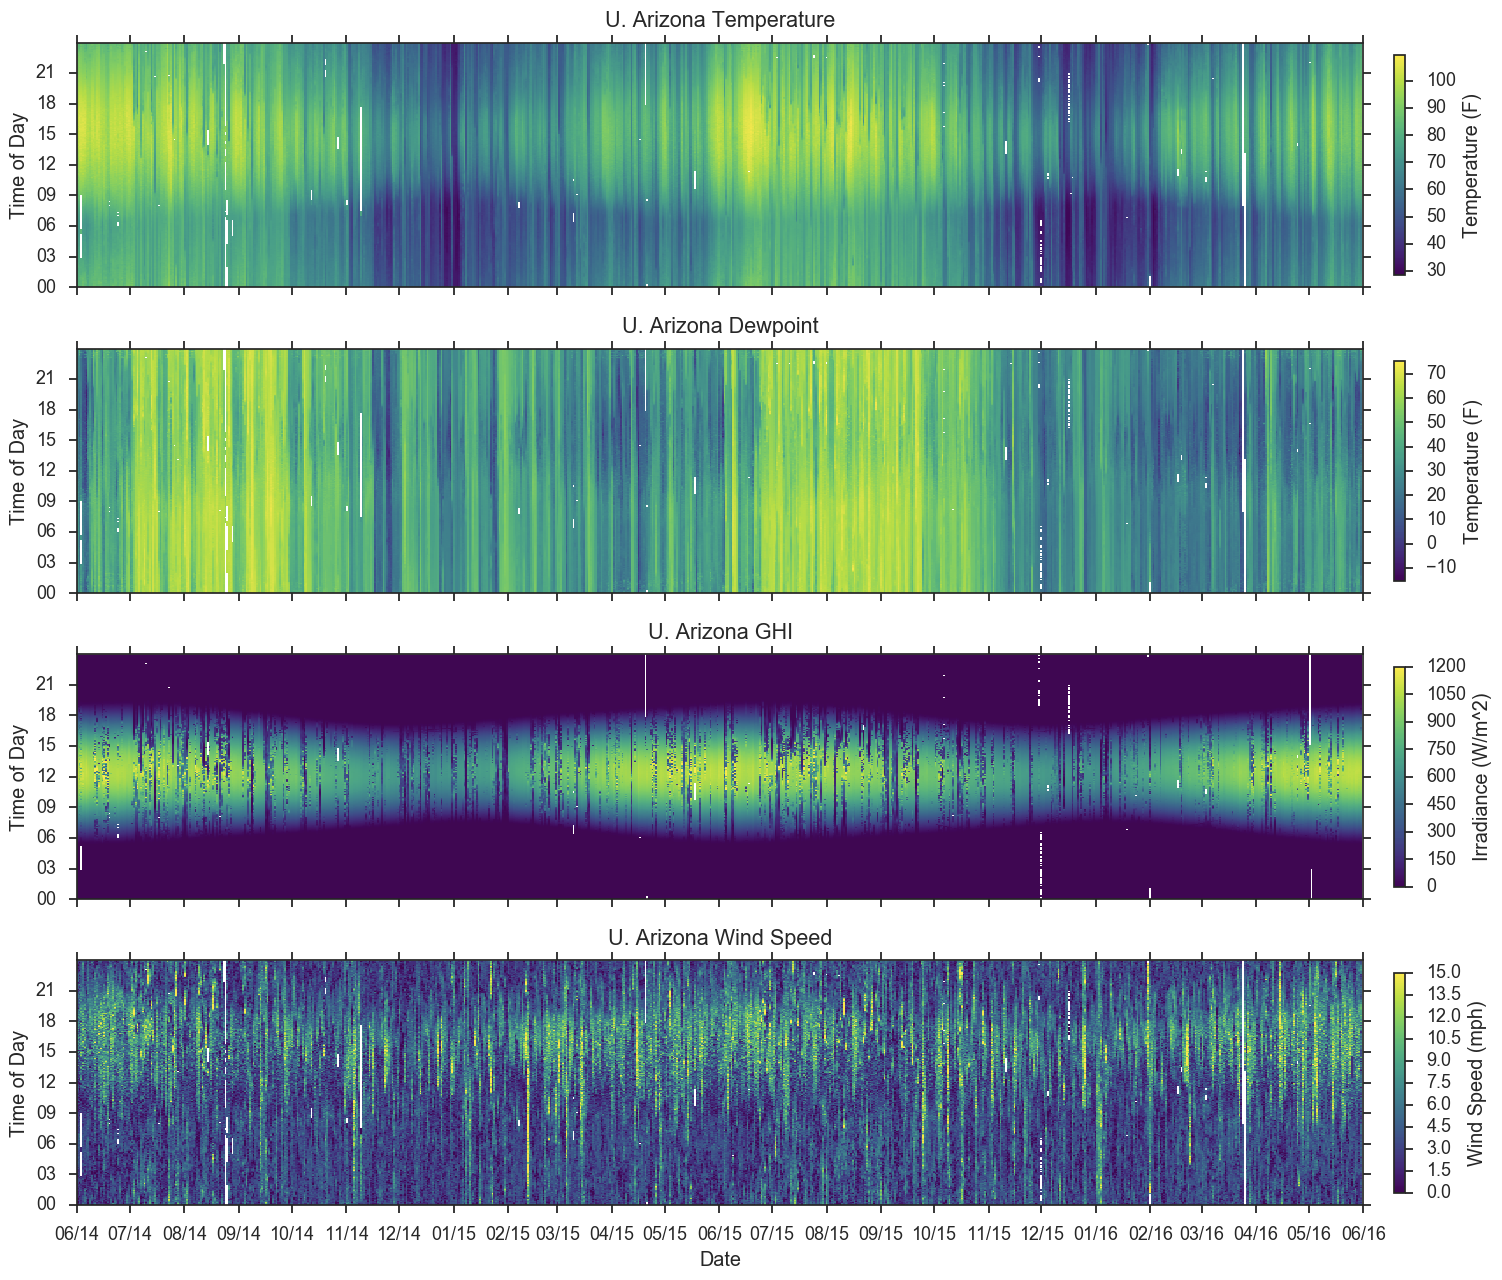
\includegraphics[width=\textwidth]{figs/ua_heat.png}
\caption[Heatmaps of temperature, dewpoint, irradiance, and wind
speed]{Time of day heatmaps for temperature, dewpoint, global
  horizontal irradiance (GHI), and wind speed all measured at the
  University of Arizona in Tucson. Notable features include the many
  clear days evident in the GHI heatmap and the beginning and end of the
  monsoon season (when moisture from the Gulf of California moves into
  Arizona) visible in the dewpoint heatmap.}
\label{fig:ua_heatmap}
\end{figure}

Utilities in Arizona are well on their way to generate 15\% of their
energy from renewable resources by 2025 as required by the Arizona
Renewable Energy Standard and Tariff \citep{rest}.
As mentioned above, DG solar systems provide a large fraction of the
total renewable energy generation.
One problem utilities encounter with DG systems is that real-time
monitoring is limited.
Since the power generated by these systems can also be consumed on
site, variability in DG power is visible to the utilities as
variability in the load.
Real-time estimates (or nowcasts) and forecasts of this DG variability
will be required for the most accurate load forecasts.

\begin{figure}[h]
\centering
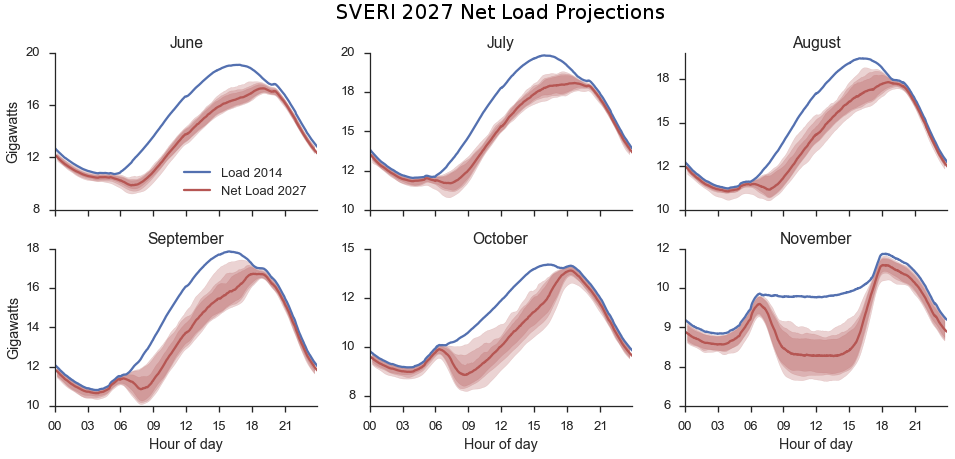
\includegraphics[width=\textwidth]{figs/duckcurves.png}
\caption[Projected SVERI 2027 duck curves]{Net load (total load minus
  wind and solar generation) projections for SVERI in 2027 if
  utilities continue business as usual. The shape of the November net
  load is referred to as a duck curve. Forecasts along with storage
  and other policies will help utilities change how solar and wind
  power are controlled to avoid these multi-GW ramps. Figure produced
  as a part of the SVERI?? report?}
\label{fig:duckcurves}
\end{figure}

Similar to DG, utilities may consider power generated at large solar
and wind power plants to be modifiers of the load instead of plants
that are controlled and dispatched.
Utilities are then interested in what they call the net load or the
total load minus the generation from solar and wind power plants.
Based on projections from 2014 SVERI data, we project net load
profiles will resemble those in \cref{fig:duckcurves}.
Notice the large power ramps that occur in the so called duck curve in
November.
Dealing with these 3 GW ramps in only a few hours would cost a great
deal if utilities rely only on the current grid technology.
Using forecasts, utilties can better control large solar and wind
power plants and avoid some of these large ramps.
Other smart grid technologies such as energy storage and time of use
rates will also play a critical role in maitaining the reliability of
the future grid.

\section{Solar Irradiance Forecasting}
nowcasting DG

Why?

Variable solar power plant fig
\begin{figure}[h]
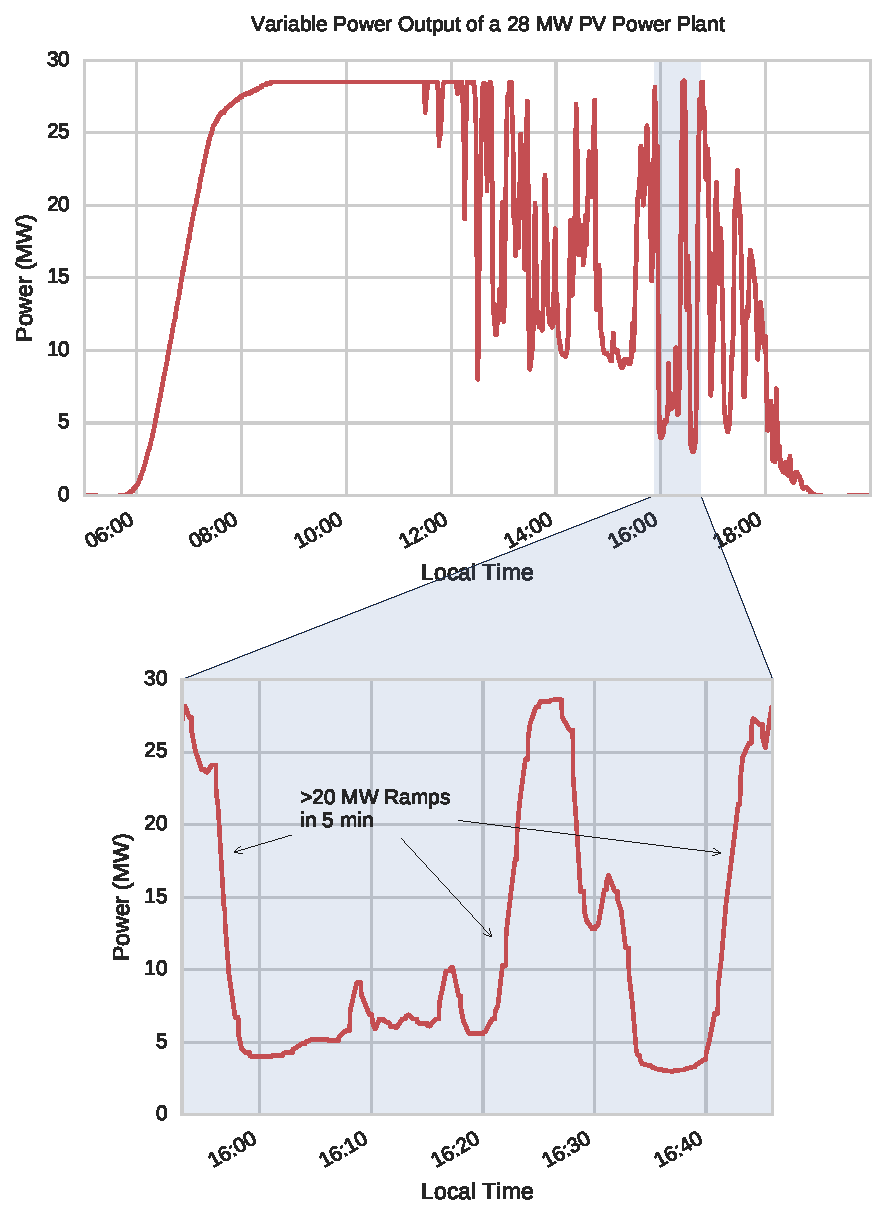
\includegraphics[width=\textwidth]{figs/avalon_ramps.pdf}
\end{figure}

other techniques

little bit about WRF

\begin{figure}[h]
\subfloat{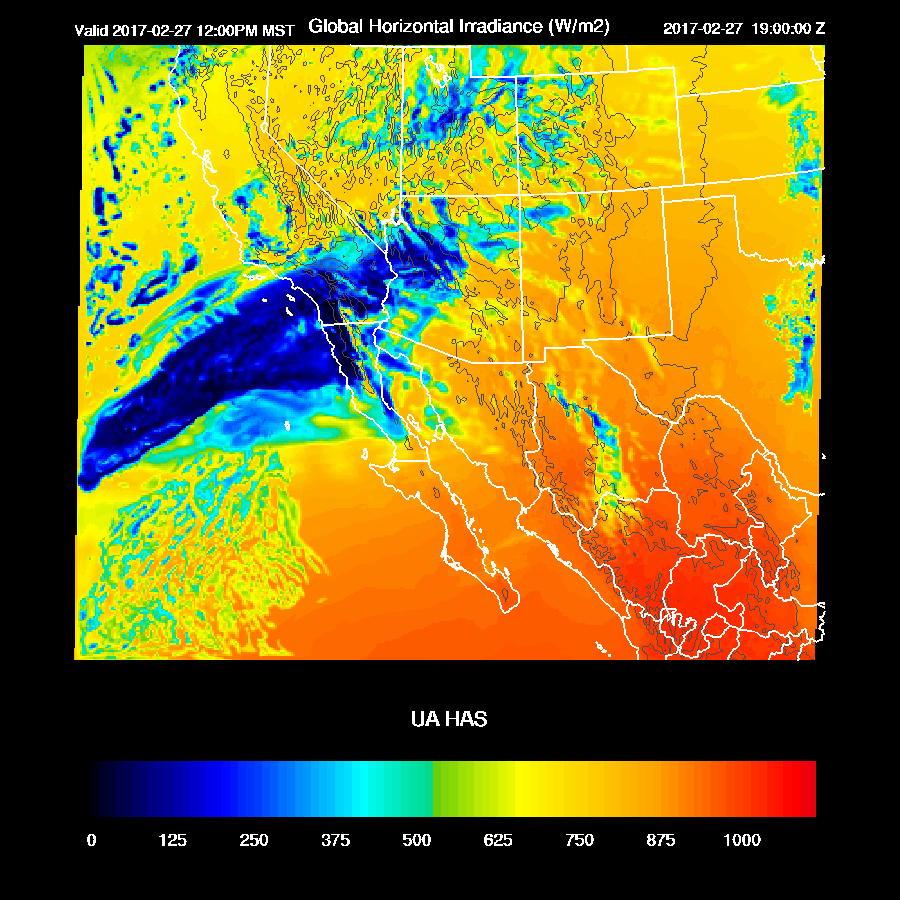
\includegraphics[width=0.5\textwidth]{figs/wrf_ghi.png}}
\hspace{-.5em}
\subfloat{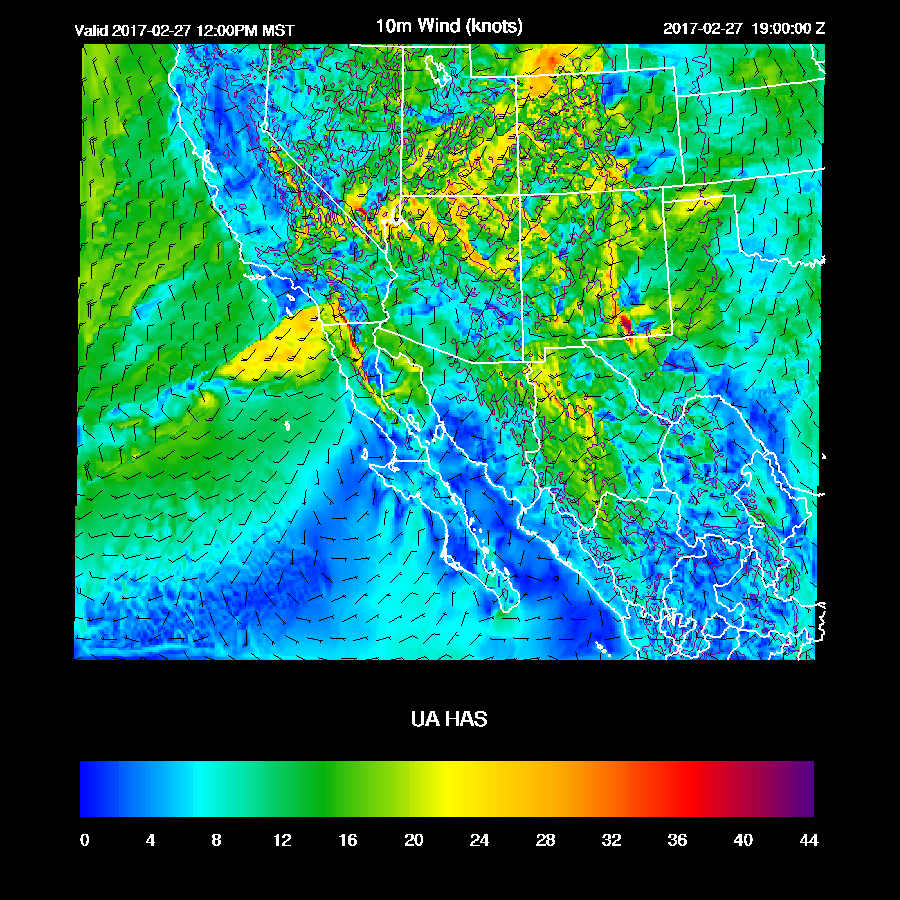
\includegraphics[width=0.5\textwidth]{figs/wrf_wind.png}}
\end{figure}


\begin{figure}[h]
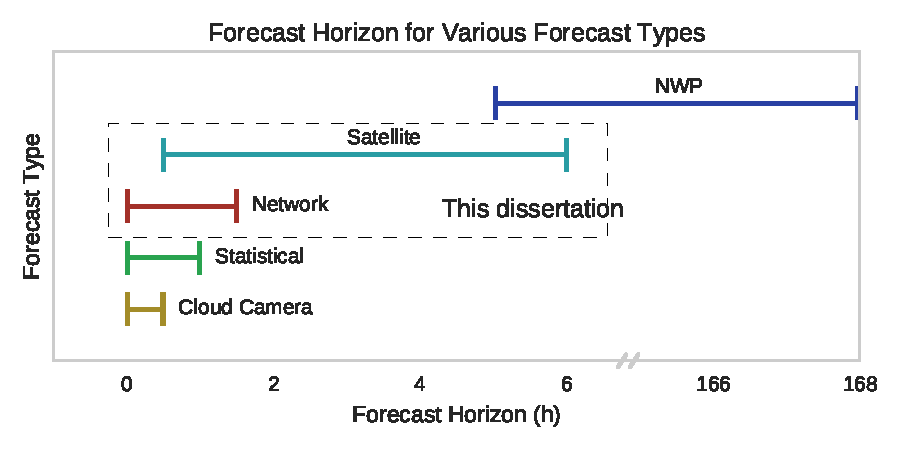
\includegraphics[width=\textwidth]{figs/fxhoriz.pdf}
\caption[Forecast horizon for various forecast types]{The optimal
  forecast horizons for various types of short-term forecasts. This
  dissertation will focus on network and satellite forecasts.}
\label{fig:fxhoriz}
\end{figure}


\section{This Dissertation in Brief}

\Cref{fig:bullshitplot} shows theoretical estimates of
forecast errors as a function of forecast horizon created near the
start of this dissertation work.
This dissertation works to analyze forecasting methods and measure
their relative errors as a function of forecast horizon in order to
produce the best forecasts for solar power in the Southwest.
\Cref{fig:newshitplot} shows the culmination of this work.
The dashed lines will beg studied in future work.

\begin{figure}[h]
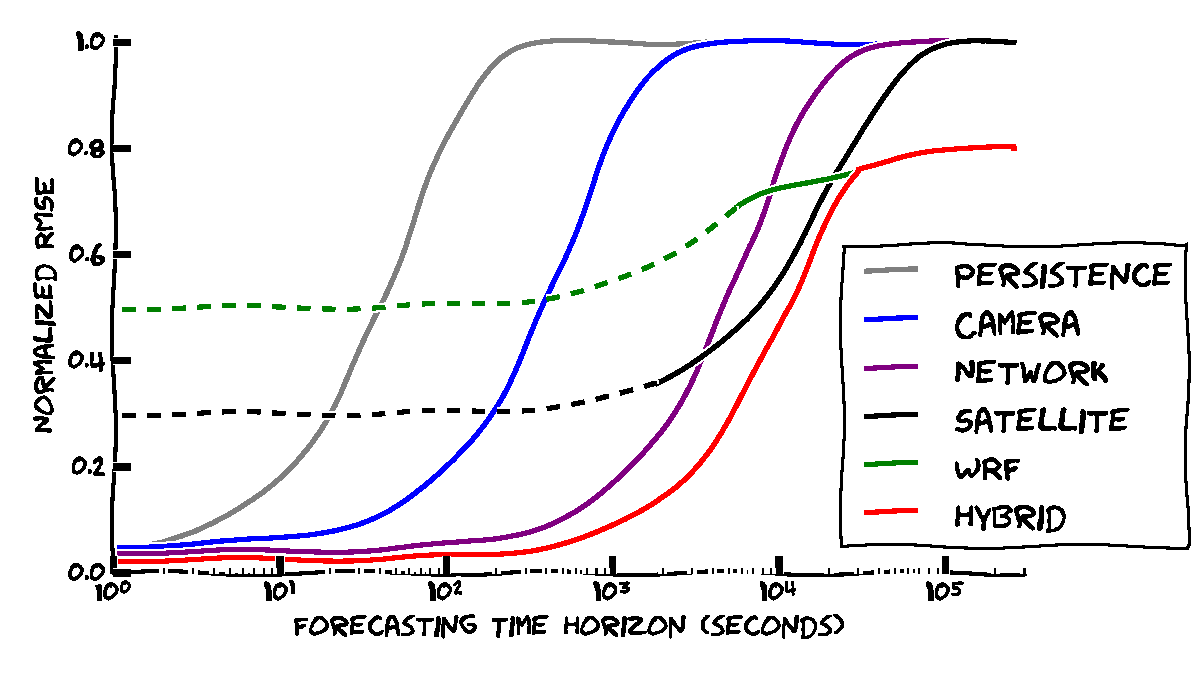
\includegraphics[width=\textwidth]{figs/bullshit.pdf}
\end{figure}

\begin{figure}[h]
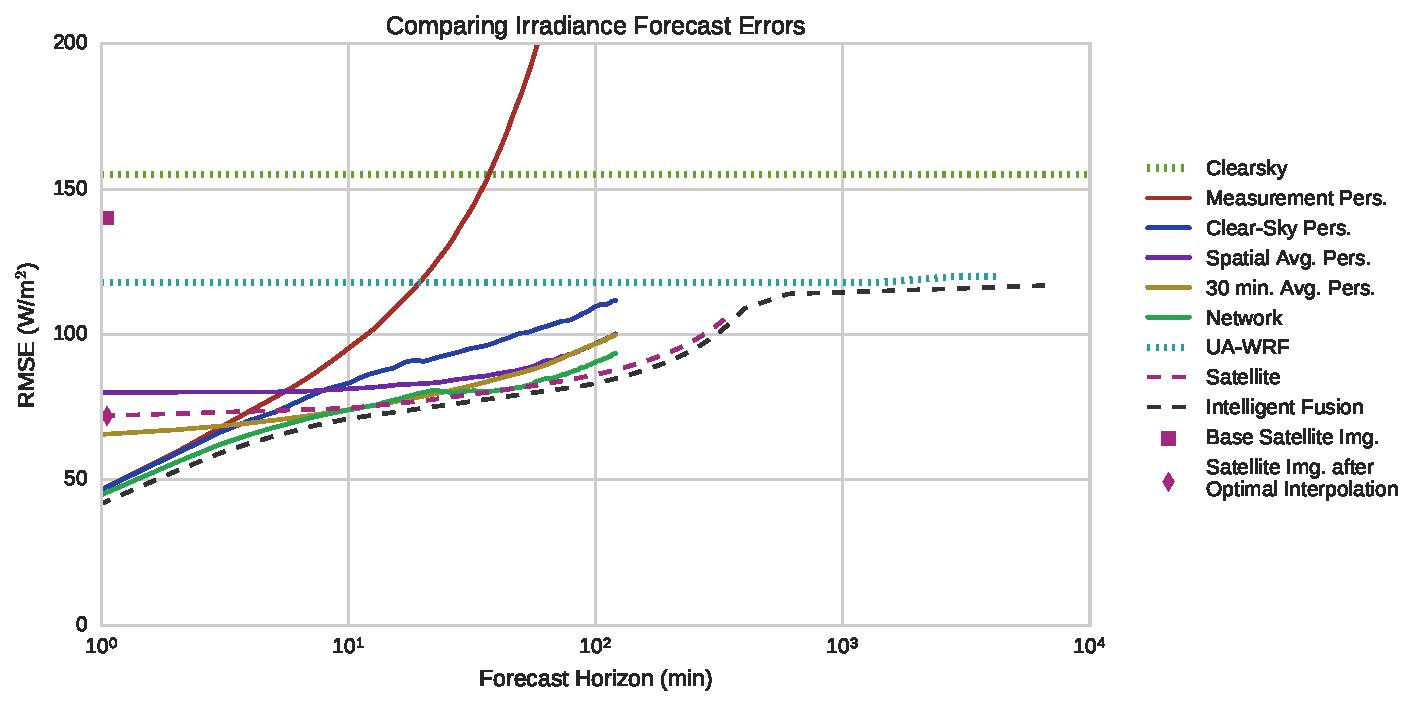
\includegraphics[width=\textwidth]{figs/timehorizon.pdf}
\caption[Irradiance forecast errors across forecast horizons]{A
  comparison of irradiance forecast root-mean squared errors (RMSE)
  across many time horizons. The solid lines (and points) indicate
  forecasts that will be studied in depth in this dissertation. Dashed
  lines are based on prelimnary analysis, but have not been studied in
  depth. Pers.\ refers to persistence, and UA-WRF refers to the
  numerical weather models generated at the UA using the Weather
  Research and Forecasting (WRF) model. The optimal grinding is a
  theoretical combination of forecasts at diffferent time horizons for
  the best forecast at all horizons. The persistence and network
  forecasts will be discussed in \Cref{chap:network} and the satellite
  image points will be discussed in \Cref{chap:satoi}.}
\label{fig:newshitplot}
\end{figure}

The specific forecasting methods studied in this dissertation rely on
a network of irradiance sensors.
A network with sufficient density and time resolution did not exist in
Tucson at the start of this dissertation work, so we set out to design
inexpensive sensors and to deploy them.
The design and deployment of the network is described in
\cref{chap:sens_net}.
For the period of April to July 2014, we collected data from about 50
custom sensors and rooftop PV systems to use in subsequent studies.

\begin{figure}[h]
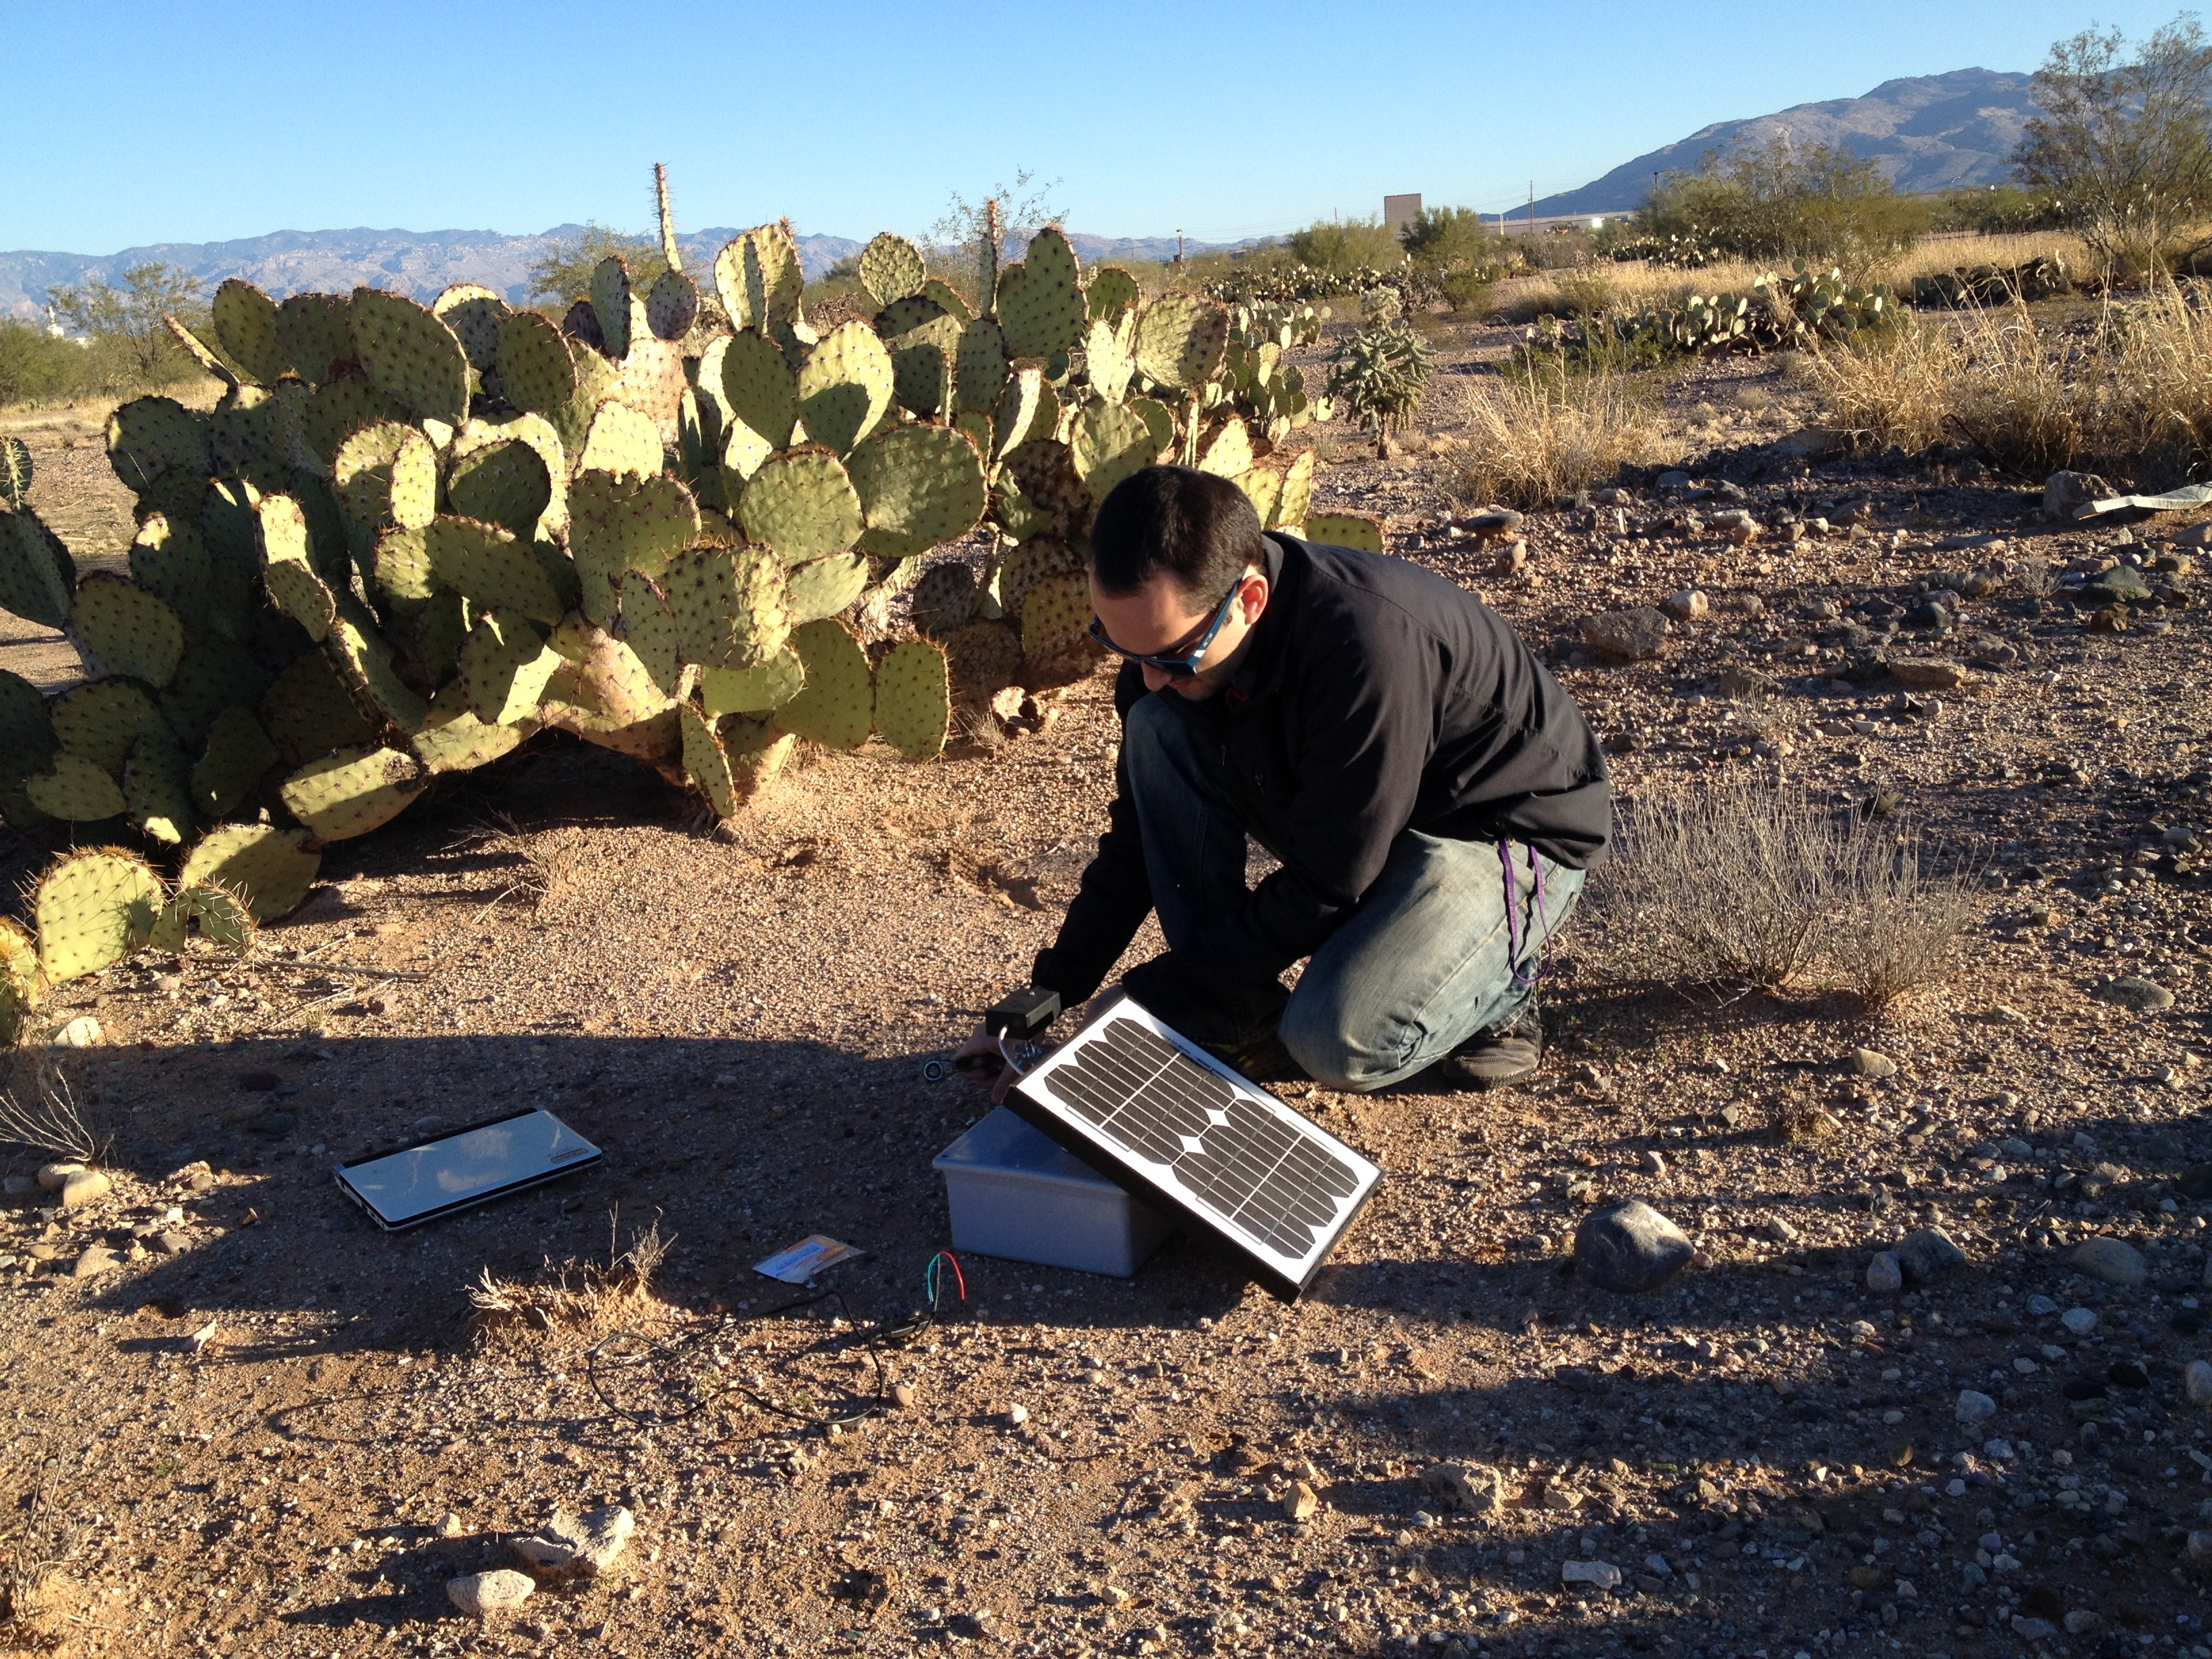
\includegraphics[width=\textwidth]{figs/sensdeploy.jpg}
\end{figure}


With this irradiance network data, the first forecasting methodology
we implemented and analyzed relies only on data from the network as
described in \cref{chap:network}.
This forecast is labeled as network in \cref{fig:newshitplot}.
On average this forecast shows a skill improvment of 20\% over a
reference persistence forecast.
The network forecast also nicely transitions from improving upon a
clear-sky persistence forecast at very short forecast horizons and an
area or time average persistence at longer horizons.

\begin{figure}[h]
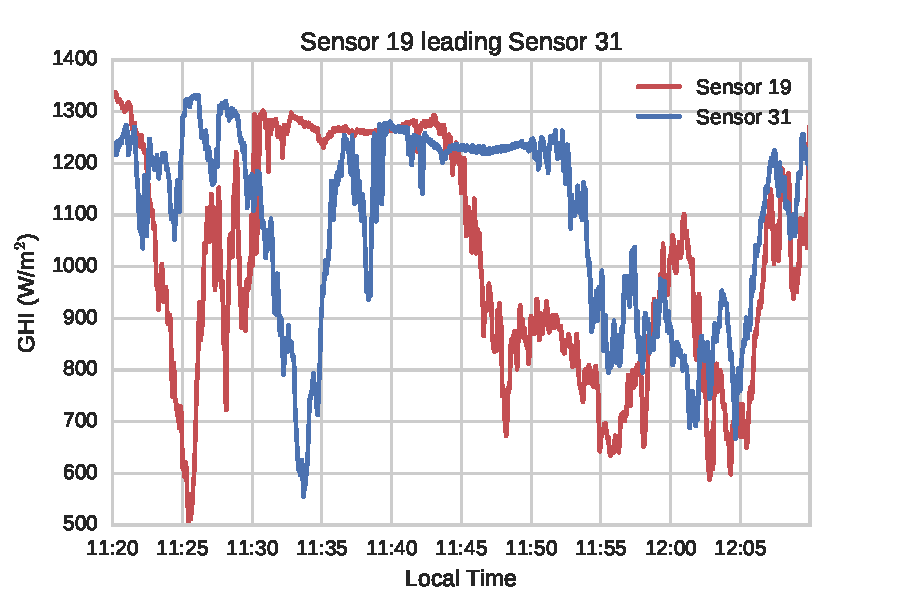
\includegraphics[width=\textwidth]{figs/leading_sens.pdf}
\end{figure}

\begin{figure}[h]
\centering
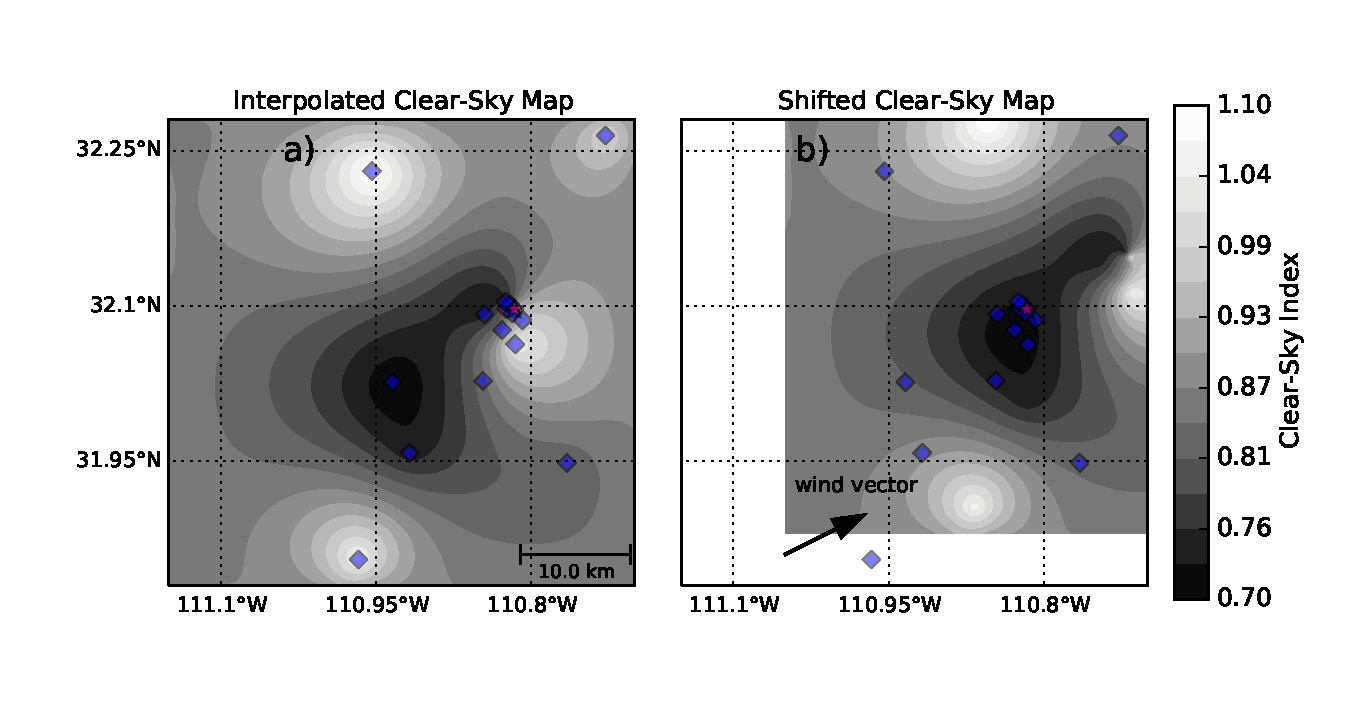
\includegraphics[width=0.96\textwidth]{figs/clearmap.pdf}
\caption{An example interpolated map of clear-sky index on 5/19/14 near noon is shown in a). Using the estimated cloud motion vectors this map is shifted according to desired forecast horizon as shown in b). Then, samples from this shifted map are taken to as the forecasted clear-sky index for a particular location. The white space at bottom and left of b) is filled in with the average clear-sky index of all sensors at the time the forecast is generated. The red star indicates the sensor that was used to evaluate forecasts.}
\label{fig:clearmap}
\end{figure}

\begin{figure}[t]
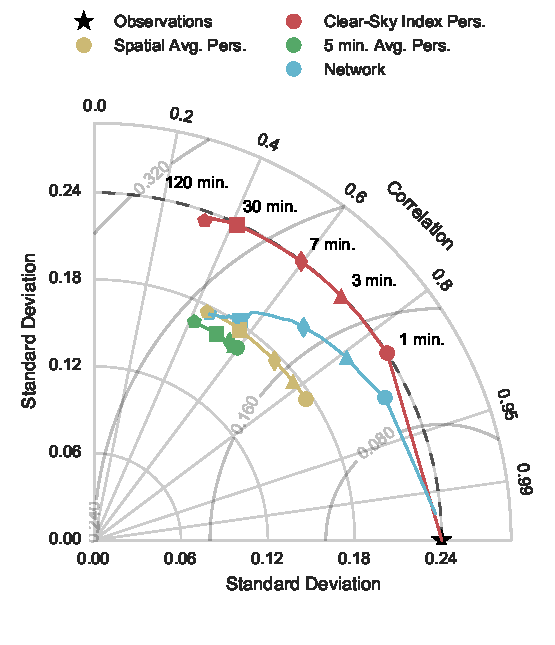
\includegraphics[width=\textwidth]{figs/taylor_diagram.pdf}
\caption{Taylor diagram for clear-sky index persistence (red), spatially-averaged persistence (yellow), 5-min time-averaged persistence (green), and network (light blue) forecasts for 1 min (circle), 3 min (triangle), 7 min (diamond), 30 min (square), and 120 min (pentagon) forecast horizons. The black dashed line indicates the standard deviation of the data. Solid contours around the observations point are lines of constant CRMSE. Forecasts for clear-sky index were used so all quantities are dimensionless. At the 120 min forecast horizon, the spatially-averaged persistence and network points overlap. Network forecasts start with a standard deviation near that of the measurements, but this decreases at longer time horizons as the network forecast begins to resemble spatially-averaged persistence.}
\label{fig:taylor}
\end{figure}

\begin{figure}[t]
 \centering
 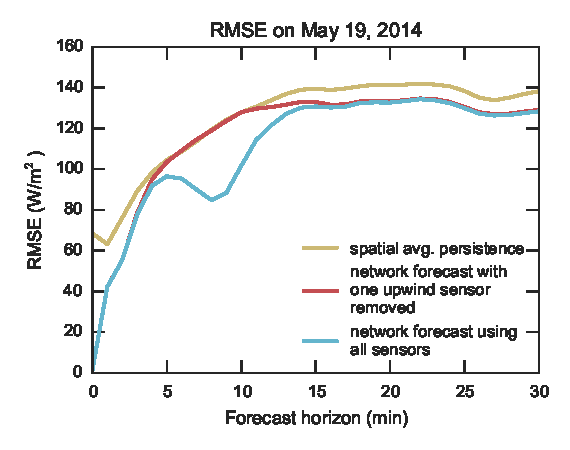
\includegraphics[width=0.9\textwidth]{figs/missing.pdf}
 \caption{RMSE vs forecast horizon on May 19, 2014 for network forecasts made with all the sensors in the network (blue) and with one upwind sensor removed (red), along with a spatially-averaged persistence forecast (yellow). The dip at 7 min for the forecast using the full network illustrates that properly placed upstream sensors do improve forecasts over a simple spatial average.}
\label{fig:circuitbreak}
\end{figure}

\begin{sidewaystable}[p]
\centering
\caption{Summary of error statistics for network forecasts for the 46 days with clouds. Error statistics were calculated for the entire dataset at once. Only forecasts and data with solar zenith angle less than $75^\circ$ were used. The mean irradiance was $\bar{y} = 662 \mbox{ W/m$^2$}$ and the mean clear-sky index was $\bar{k} = 0.92$.}
\begin{tabular}{llllllll}
\toprule
FH &  rMAE (\%) &  MAE (W/m$^2$) &  MBE (W/m$^2$) &  rRMSE (\%) &  RMSE (W/m$^2$) &  Avg. skill (\%) \\
\midrule
 1 min  &      4.96 &          30.97 &          -1.44 &      11.90 &           82.55 &           22.96 \\
 3 min  &      7.51 &          48.13 &          -1.39 &      15.89 &          110.46 &           23.09 \\
 5 min  &      9.29 &          59.59 &          -3.91 &      18.67 &          127.06 &           19.65 \\
10 min  &     11.39 &          71.38 &          -8.59 &      22.11 &          141.44 &           18.63 \\
20 min  &     13.23 &          82.39 &         -10.46 &      24.03 &          152.84 &           18.66 \\
30 min  &     13.95 &          86.57 &          -7.52 &      24.49 &          154.15 &           21.21 \\
60 min  &     15.45 &          95.59 &          -6.65 &      26.59 &          160.72 &           21.00 \\
120 min &     17.02 &         106.51 &          -2.01 &      29.20 &          172.45 &           19.58 \\
\bottomrule
\end{tabular}
\label{table:network_errors_cloudy}
\end{sidewaystable}




While analyzing this network forecast, we also carefully analyzed
various types of persistence forecasts to understand how the network
forecast works.
We found that smoother forecasts, or those with lower variance as
compared to the observations, may seem to perform better than
forecasts with higher variance when error metrics are considered in
isolation.
Using a Taylor diagram, we show that network forecasts transition from
matching the observation's variance to essentially becoming an area
average persistence forecast after about 20 minutes.

With short-term forecasts covered by the network forecasts, we began
studying forecasts derived from satellite images.
A number of algorithms exist that convert images of the tops of clouds
from geostationary satellites to images of irradiance on the ground.
Naturally, this conversion from cloud top brightness to the amount of
radiation that passes through clouds is error prone.
We found that these satellite derived irradiance estimates from a
current image (pink square on left axis of \cref{fig:newshitplot}),
before any forecasting is involved, had errors nearly as large as
always assuming a clear sky.
It is unlikely that producing a forecast from such a nowcast would
reduce errors, so satellite derived forecasts would quickly become
worse than a clear-sky forecast, at least in terms of RMSE.
Thus, in order to produce high quality forcasts from satellite derived
irradiance images, we first improved the satellite derived irradiance
nowcasts.

\begin{figure}[h]
\subfloat{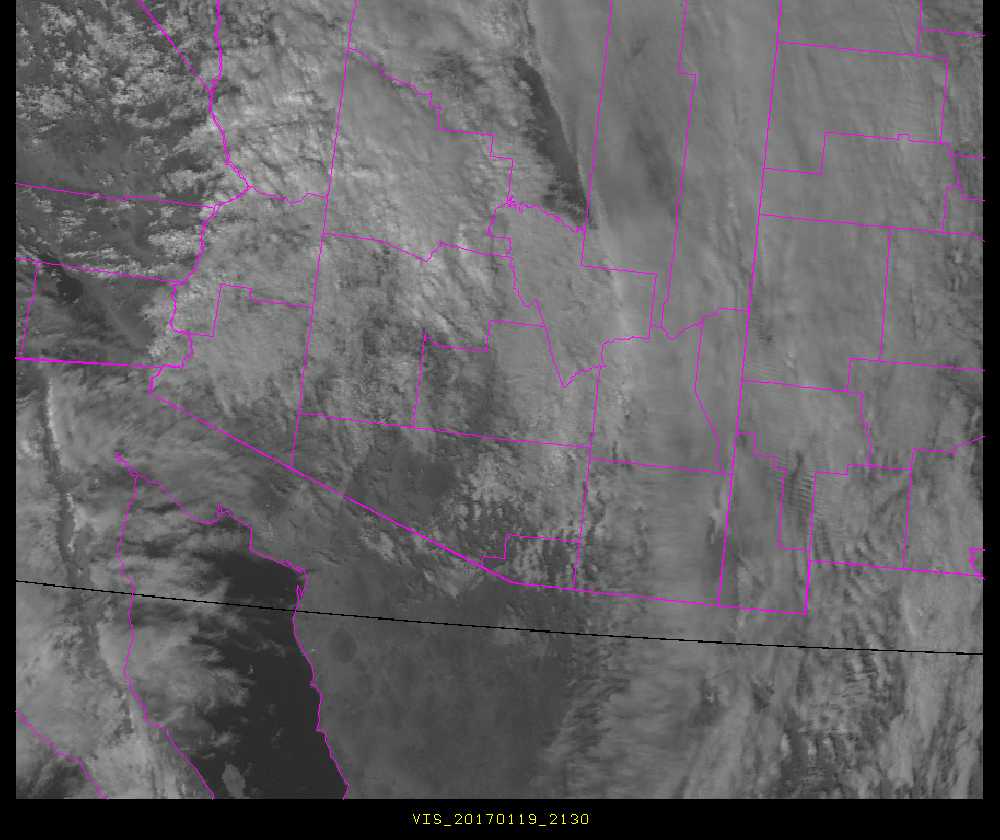
\includegraphics[width=0.5435\textwidth]{figs/rawvis.png}}
\subfloat{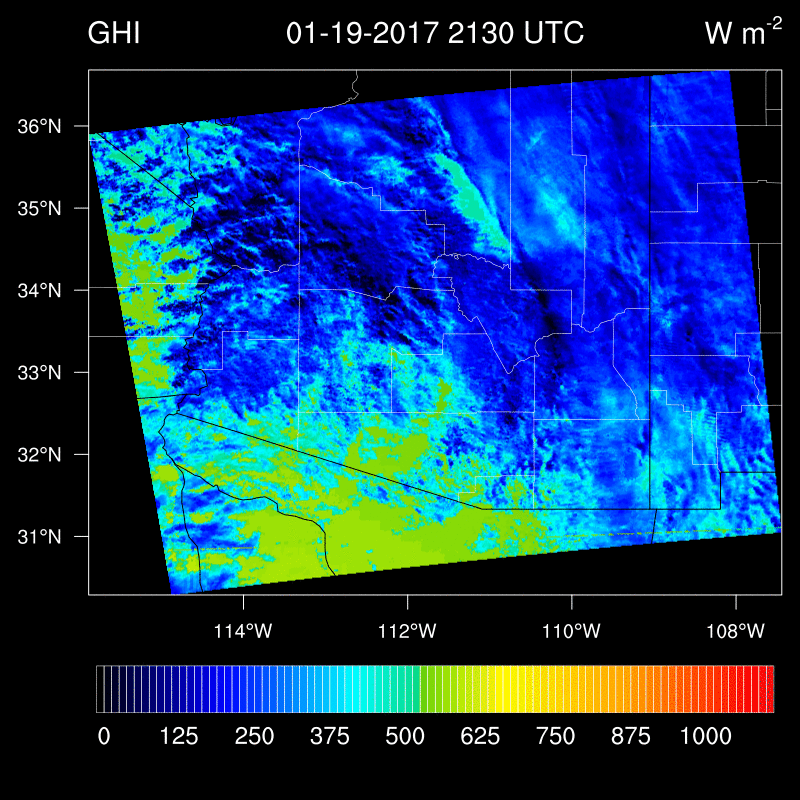
\includegraphics[width=0.4565\textwidth]{figs/satirr.png}}
\end{figure}

\begin{figure}[h]
\centering
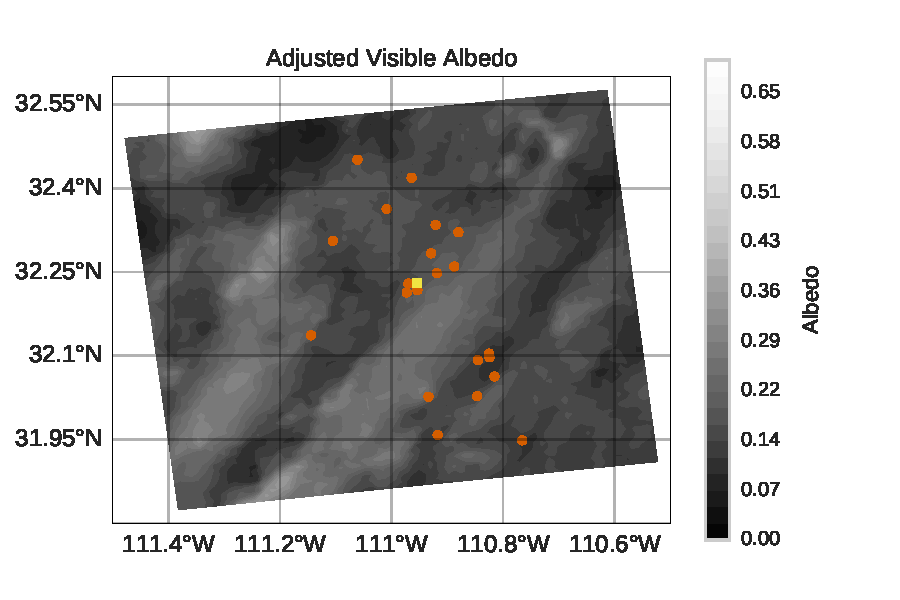
\includegraphics[width=0.5\textwidth]{figs/pa.pdf}
\caption{Visible albedo image derived from the visible channel of the
  GOES-W satellite. Lighter colors indicate cloudier areas. The orange
  dots represent the locations of the sensors used in this study which
  includes both irradiance sensors and rooftop PV systems as described
  in \cref{sec:data}. The yellow square in the center indicates the
  location of a calibrated GHI sensor on the University of Arizona
  campus. The image covers an area of roughly $75 \times 80$ km over
  Tucson, AZ.}
\label{fig:vis}
\end{figure}

\begin{figure}[h]
\centering
\captionsetup[subfigure]{labelformat=empty}
\subfloat{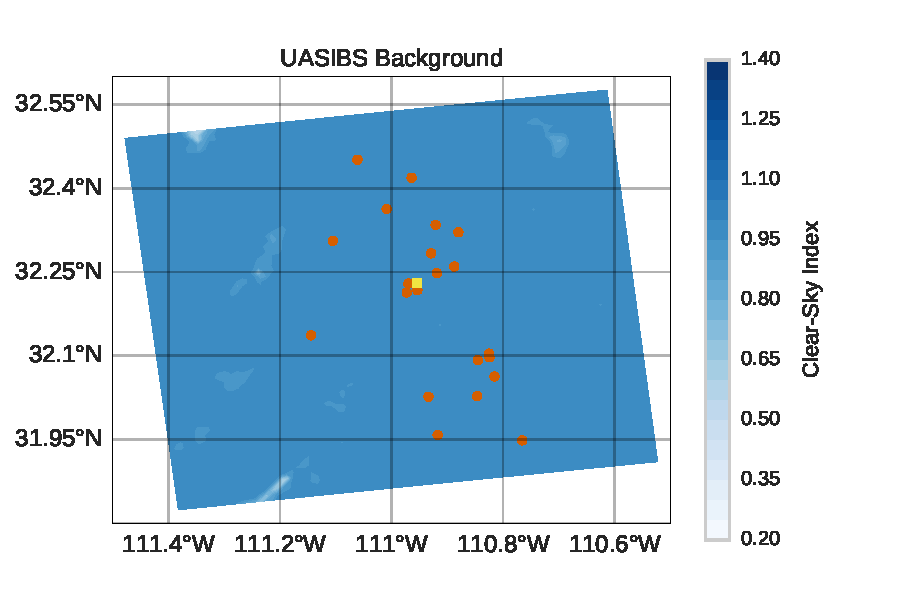
\includegraphics[width=0.5\textwidth]{figs/uasibs_bck_ex.pdf}}
\subfloat{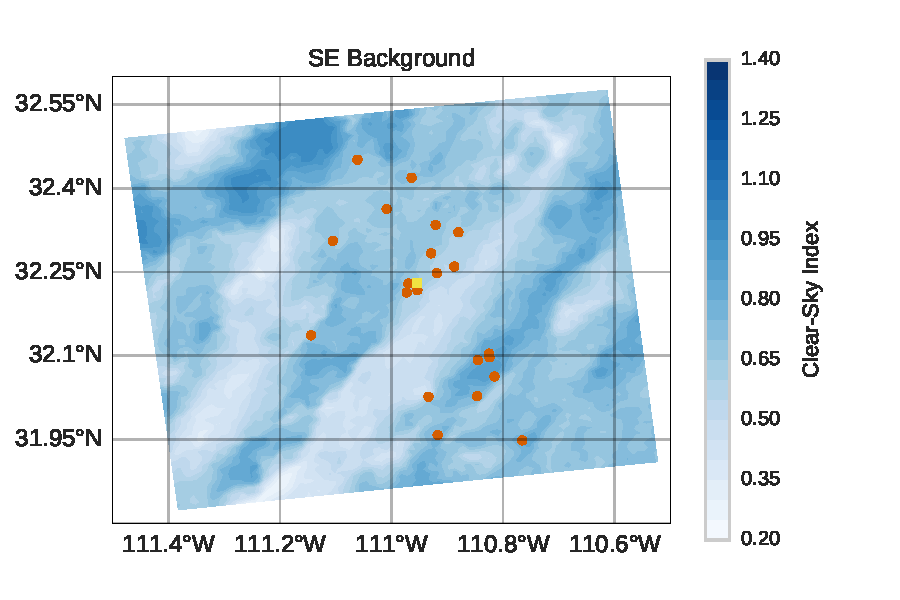
\includegraphics[width=0.5\textwidth]{figs/suny_bck_ex.pdf}}
\vspace{-1em}\\
\subfloat{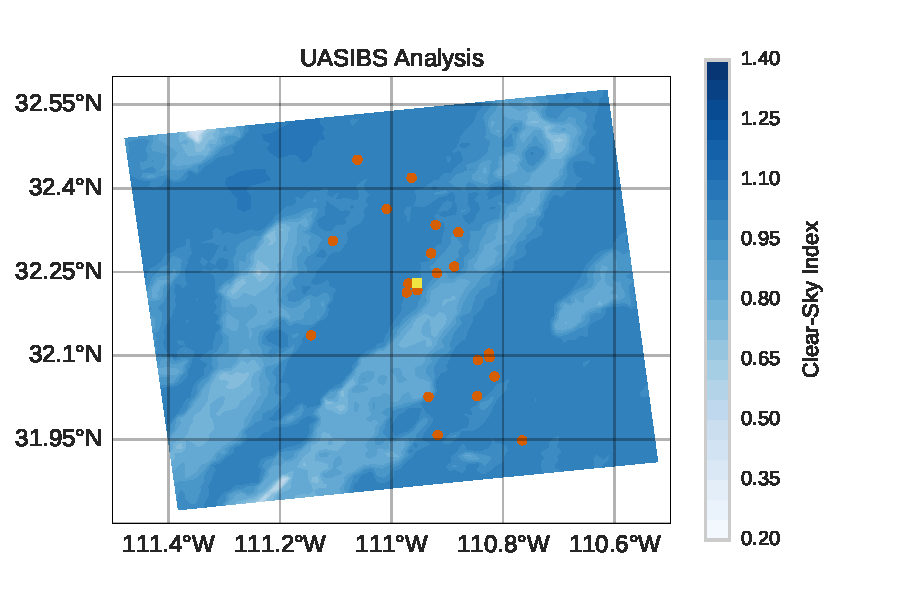
\includegraphics[width=0.5\textwidth]{figs/uasibs_anl_ex.pdf}}
\subfloat{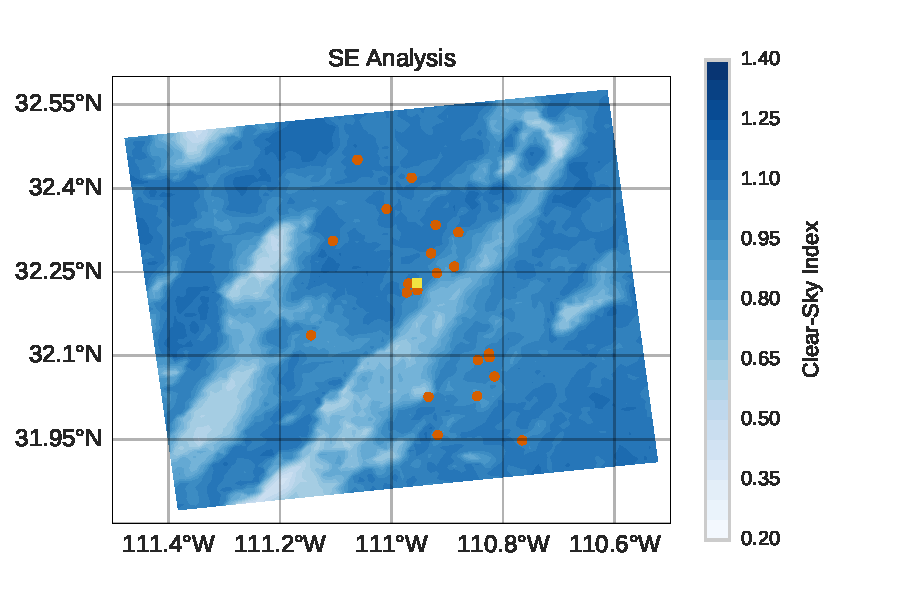
\includegraphics[width=0.5\textwidth]{figs/suny_anl_ex.pdf}}
\caption{Example background (top row) and analysis (bottom row)
  clear-sky index images using the UASIBS (left column) and SE (right
  column) satellite image to ground irradiance models applied to the
  visible satellite image shown in \cref{fig:vis}. Note that in this
  case, UASIBS failed to produce many clouds. OI adds clouds to the
  analysis and also makes the darker, clear areas even more clear.  In
  this case, the SE model overproduces clouds. OI reduces the cloud
  amount while keeping clouds in suitable locations.}
\label{fig:oi_example}
\end{figure}

\begin{table}[htbp]
  \caption{Error statistics for the NREL MIDC sensor on the University
    of Arizona campus. The analysis was computed with only the MIDC
    sensor withheld and averaged over the verification data set, and
    cloudiness covariance was used. Both the
    UASIBS and SE models show improvements and have a similar
    analysis RMSE\@. Units are W/m$^2$.}
\label{table:irr}
\vspace{0.5em}
\input{figs/ghi_err_table}
\centering
\end{table}


Better satellite derived irradiance nowcasts were generated by again
using data from the irradiance sensor network as described in
\cref{chap:satoi}.
Using a data assimilation method known as optimal interpolation, we
combined the sensor data with the satellite derived irradiance based
on the relative errors between them.
We also parameterized the correlations between pixels in the satellite
images in various ways.
These correlations are responsible for spreading information from the
sensor locations to other locations throughout the image.

We found significant improvements using this method after various
complicating factors such as misalignment in the satellite image
relative to the ground sensors were corrected.
The improved nowcasts RMSE is shown as the pink diamond in
\cref{fig:newshitplot} and is almost half of the RMSE for the
uncorrected images.
We also found that this method to improve satellite irradiance
nowcasts is applicable to a number of satellite to irradiance
algorithms.

To produce forecasts of irradiance in future work, one might use a
forecasting method that relies on only cloud advection.
With a forecasting model in place, optimal interpolation can be
extended to the Kalman filter with constantly incorporates new data
into a forecast while also retaining information about past data.
It is common in numerical weather prediction to use an ensemble of
states to propogate and Kalman filter.
An ensemble in this case also allows for each forecast to have a
different cloud motion field which may improve the final forecasts.

Satellite forecasts have been shown to perform well for forecast
horizons up to 6 hours.
For longer forecast horizons, numerical weather models are likely
needed.
We currently run the Weather Research and Forecasting (WRF) model with
a custom configuration for Arizona.
Improvements in the WRF model may come from assimilating satellite
data, data from the sensor network, or studying WRF ensembles.


Finally, once high-quality forecasts are available for all forecast
horizons, they can be intellgently fused to produce a single forecast
that incorporates the best properties of each forecast methodology.
Utilities and other stakeholders often need these fused forecasts to
make decisions.





%%% Local Variables:ah
%%% mode: latex
%%% TeX-master: "dissertation"
%%% End:
